\documentclass{standalone}
\usepackage{pgfplots}
\usepackage{bm}
\usepackage{siunitx}
\pgfplotsset{compat=1.12}
\usetikzlibrary{arrows, decorations.pathmorphing, backgrounds, positioning,fit,petri}
\usetikzlibrary{calc}

\newcommand{\xdistl}{6cm}
\newcommand{\xdistr}{4cm}

\begin{document}

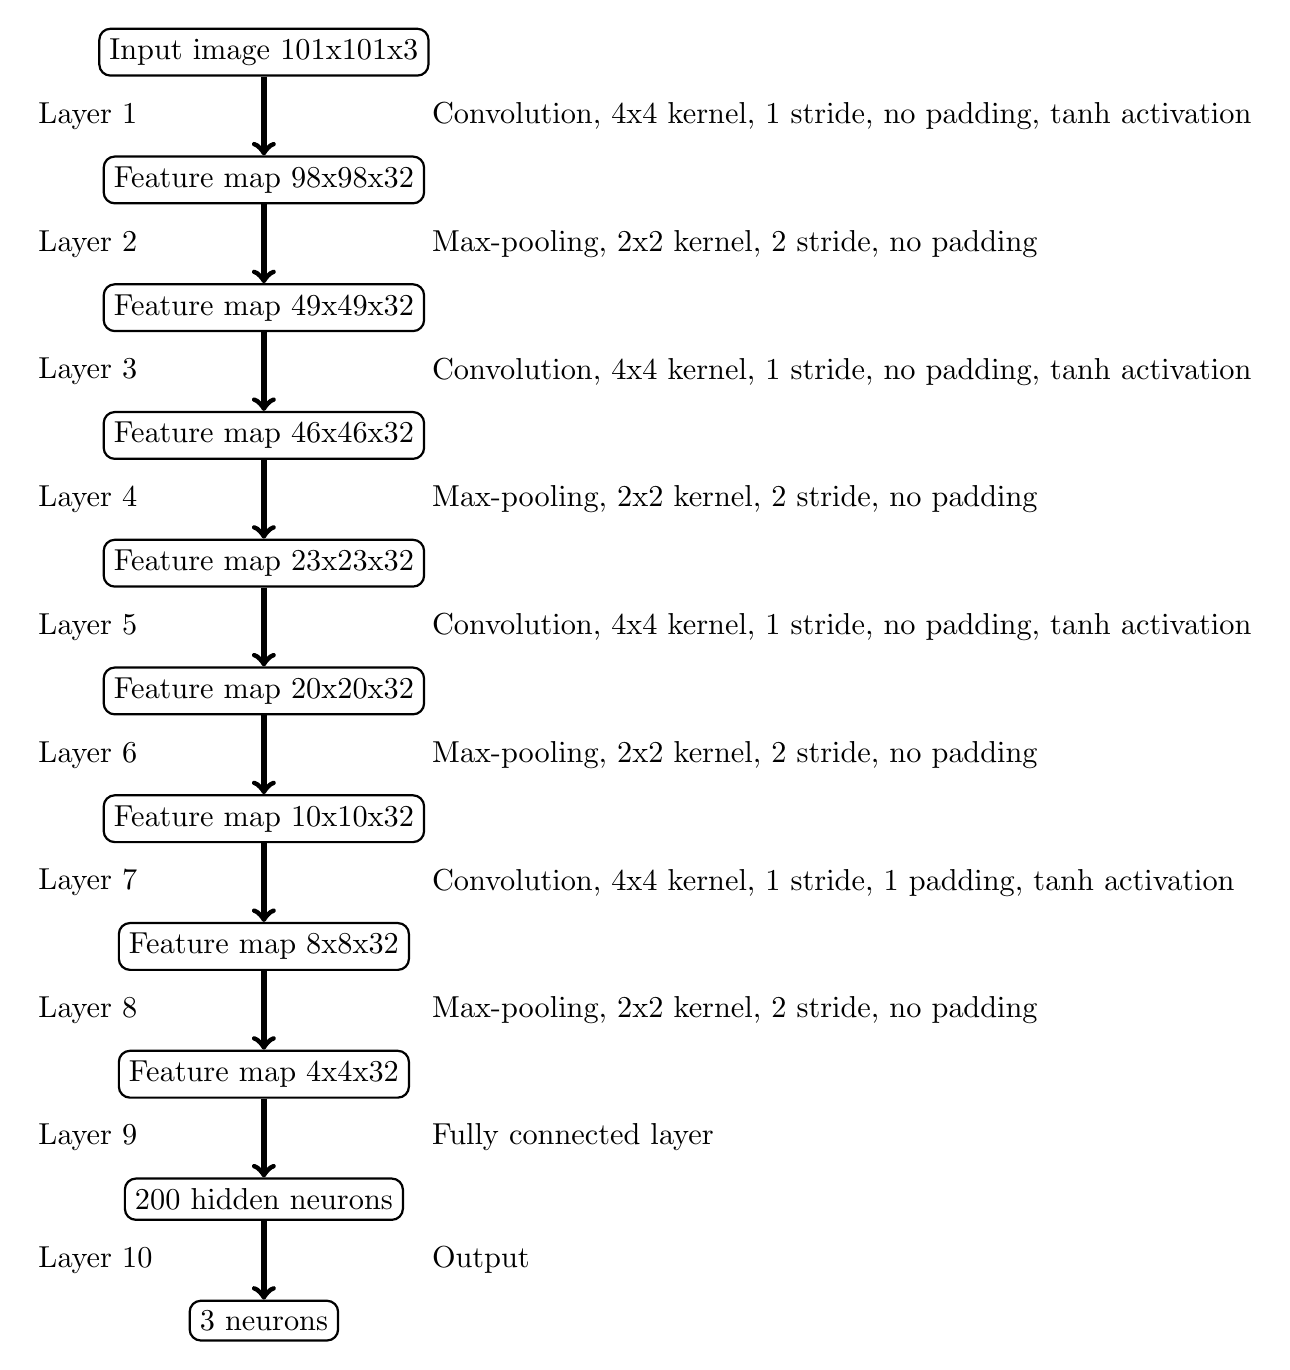
\begin{tikzpicture}
  \fontsize{11}{11}
  {
    \node[black, draw, thick, rounded corners] (f1) at (0, 0) {Input image 101x101x3};
    \node[black, draw, thick, rounded corners] (f2) [below=of f1] {Feature map 98x98x32};
    \node[black, draw, thick, rounded corners] (f3) [below=of f2] {Feature map 49x49x32};
    \node[black, draw, thick, rounded corners] (f4) [below=of f3] {Feature map 46x46x32};
    \node[black, draw, thick, rounded corners] (f5) [below=of f4] {Feature map 23x23x32};
    \node[black, draw, thick, rounded corners] (f6) [below=of f5] {Feature map 20x20x32};
    \node[black, draw, thick, rounded corners] (f7) [below=of f6] {Feature map 10x10x32};
    \node[black, draw, thick, rounded corners] (f8) [below=of f7] {Feature map 8x8x32};
    \node[black, draw, thick, rounded corners] (f9) [below=of f8] {Feature map 4x4x32};
    \node[black, draw, thick, rounded corners] (f10) [below=of f9] {200 hidden neurons};
    \node[black, draw, thick, rounded corners] (f11) [below=of f10] {3 neurons};



    \draw[->, line width=2pt] (f1.south) -| (f2.north);
    \draw[->, line width=2pt] (f2.south) -| (f3.north);
    \draw[->, line width=2pt] (f3.south) -| (f4.north);
    \draw[->, line width=2pt] (f4.south) -| (f5.north);
    \draw[->, line width=2pt] (f5.south) -| (f6.north);
    \draw[->, line width=2pt] (f6.south) -| (f7.north);
    \draw[->, line width=2pt] (f7.south) -| (f8.north);
    \draw[->, line width=2pt] (f8.south) -| (f9.north);
    \draw[->, line width=2pt] (f9.south) -| (f10.north);
    \draw[->, line width=2pt] (f10.south) -| (f11.north);



    \node[black, draw, opacity=0, text opacity=1, anchor=west] (l1) at ( $ (f1)!0.5!(f2) + (2, 0)$ ) {Convolution, 4x4 kernel, 1 stride, no padding, tanh activation};
    \node[black, draw, opacity=0, text opacity=1, anchor=west] (l2) at ( $ (f2)!0.5!(f3) + (2, 0)$ ) {Max-pooling, 2x2 kernel, 2 stride, no padding};
    \node[black, draw, opacity=0, text opacity=1, anchor=west] (l3) at ( $ (f3)!0.5!(f4) + (2, 0)$ ) {Convolution, 4x4 kernel, 1 stride, no padding, tanh activation};
    \node[black, draw, opacity=0, text opacity=1, anchor=west] (l4) at ( $ (f4)!0.5!(f5) + (2, 0)$ ) {Max-pooling, 2x2 kernel, 2 stride, no padding};
    \node[black, draw, opacity=0, text opacity=1, anchor=west] (l5) at ( $ (f5)!0.5!(f6) + (2, 0)$ ) {Convolution, 4x4 kernel, 1 stride, no padding, tanh activation};
    \node[black, draw, opacity=0, text opacity=1, anchor=west] (l6) at ( $ (f6)!0.5!(f7) + (2, 0)$ ) {Max-pooling, 2x2 kernel, 2 stride, no padding};
    \node[black, draw, opacity=0, text opacity=1, anchor=west] (l7) at ( $ (f7)!0.5!(f8) + (2, 0)$ ) {Convolution, 4x4 kernel, 1 stride, 1 padding, tanh activation};
    \node[black, draw, opacity=0, text opacity=1, anchor=west] (l8) at ( $ (f8)!0.5!(f9) + (2, 0)$ ) {Max-pooling, 2x2 kernel, 2 stride, no padding};
    \node[black, draw, opacity=0, text opacity=1, anchor=west] (l9) at ( $ (f9)!0.5!(f10) + (2, 0)$ ) {Fully connected layer};
    \node[black, draw, opacity=0, text opacity=1, anchor=west] (l10) at ( $ (f10)!0.5!(f11) + (2, 0)$ ) {Output};



    \node[black, draw, opacity=0, text opacity=1, anchor=west] (ll1) at ( $ (f1)!0.5!(f2) - (3, 0)$ ) {Layer 1};
    \node[black, draw, opacity=0, text opacity=1, anchor=west] (ll2) at ( $ (f2)!0.5!(f3) - (3, 0)$ ) {Layer 2};
    \node[black, draw, opacity=0, text opacity=1, anchor=west] (ll3) at ( $ (f3)!0.5!(f4) - (3, 0)$ ) {Layer 3};
    \node[black, draw, opacity=0, text opacity=1, anchor=west] (ll4) at ( $ (f4)!0.5!(f5) - (3, 0)$ ) {Layer 4};
    \node[black, draw, opacity=0, text opacity=1, anchor=west] (ll5) at ( $ (f5)!0.5!(f6) - (3, 0)$ ) {Layer 5};
    \node[black, draw, opacity=0, text opacity=1, anchor=west] (ll6) at ( $ (f6)!0.5!(f7) - (3, 0)$ ) {Layer 6};
    \node[black, draw, opacity=0, text opacity=1, anchor=west] (ll7) at ( $ (f7)!0.5!(f8) - (3, 0)$ ) {Layer 7};
    \node[black, draw, opacity=0, text opacity=1, anchor=west] (ll8) at ( $ (f8)!0.5!(f9) - (3, 0)$ ) {Layer 8};
    \node[black, draw, opacity=0, text opacity=1, anchor=west] (ll9) at ( $ (f9)!0.5!(f10) - (3, 0)$ ) {Layer 9};
    \node[black, draw, opacity=0, text opacity=1, anchor=west] (ll10) at ( $ (f10)!0.5!(f11) - (3, 0)$ ) {Layer 10};

}
\end{tikzpicture}

\end{document} 
